\documentclass[10pt, a4paper,spanish]{article}

\usepackage[utf8]{inputenc}
\usepackage[spanish]{babel}

\usepackage[T1]{fontenc}

\usepackage[hmarginratio=1:1,top=32mm,columnsep=20pt]{geometry}
\usepackage[hang, small,labelfont=bf,up,textfont=it,up]{caption}

\usepackage{float}

\usepackage{amsmath}

\usepackage{listings}

\usepackage{enumitem}

\usepackage{hyperref}

\usepackage{graphicx}

\usepackage[most]{tcolorbox}
\usepackage{minibox}

\usepackage{titlesec}
\renewcommand\thesection{\Roman{section}}
\renewcommand\thesubsection{\Roman{subsection}}
\titleformat{\section}[block]{\large\scshape\centering}{\thesection.}{1em}{}
\titleformat{\subsection}[block]{\large}{\thesubsection.}{1em}{}

\usepackage{fancyhdr}
\pagestyle{fancy}
\fancyhead{}
\fancyfoot{}
\fancyhead[C]{ \today \ $\bullet$ Grámaticas y Lenguajes Formales $\bullet$ Práctica 2}
\fancyfoot[RO]{\thepage}

%-------------------------------------------------------------------------------
%	Seccion titulo
%-------------------------------------------------------------------------------

\title{\vspace{-15mm}\fontsize{24pt}{10pt}\selectfont\textbf{Resumen de ficheros HTML}}

\author{
	Iván López de Munain Quintana
}

\date{\today}



%-------------------------------------------------------------------------------
\begin{document}

	\maketitle % Insert title

	\thispagestyle{fancy} % All pages have headers and footers


%-------------------------------------------------------------------------------
%	TEXT
%-------------------------------------------------------------------------------



\textbf{\section{Introducción.\\\\}}

\paragraph{}
\noindent \\ En esta primera entrega se va a poner en práctica los conocimientos adquiridos de  \textit{Lex} para llevar a cabo un análisis léxico de ficheros HTML. Para realizar estos objetivos se va a descargar los ficheros HTML de las siguientes páginas: 
\begin{itemize}
    \item \url{ https://campusvirtual.uva.es}
    \item \url{https://www.wikipedia.org/}
\end{itemize}
 \noindent Para conseguir esto se ha implementado el correspondiente \textit{Makefile} con el fin de automatizar la generación del ejecutable, limpieza de carpetas y ficheros temporales y la descarga de los ya comentados HTML. Dicho \textit{Makefile} tiene la siguiente forma: \\

\begin{figure}[H]
  \centering
    \fbox{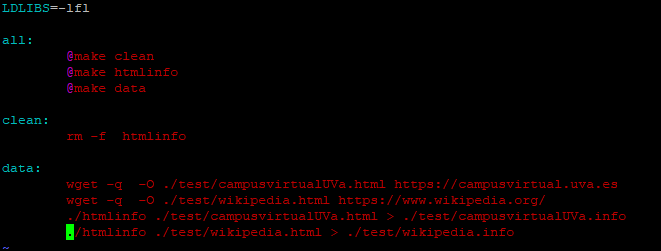
\includegraphics[width=0.75 \textwidth]{Captura.PNG}}
  \caption{Composición del \textit{Makefile}.}
\end{figure}

\noindent Podemos observar en la Figura 1 que lo primero que se lleva a cabo es el borrado del fichero que se crea al compilar y ejecutar \textit{htmlinfo.l} (\textit{htmlinfo}). Posteriormente se compila dicho fichero \textit{htmlinfo}, se descargan los fichero HTML correspondiente en donde \textit{-q} sirve para que no nos imprima notificaciones innecesarias y \textit{-O} para almacenar el HTML como fichero. Por último se ejecuta el archivo en cuesión pasándole como entrada el HTML correspondiente y almacenando el resultado en \textit{./test/campusvirtualUVa.info} y \textit{./test/wikipedia.info}.\\
\newpage
\textbf{\section{Especificaciones.\\\\}}

\noindent \\ Para lograr evitar los comentarios en HTML he reutilizado parte de una función realizada en clase llamada \textit{IgnoraComentarioMultiLinea}. Antes de nada hay que tener en cuenta que los comentarios en HTML son de la siguiente forma:
\begin{lstlisting}

    <!-- Esto es un comentario -->
    
\end{lstlisting}

\noindent \\ Es por esto que en la parte de ordenes he incluido la siguiente expresión regular para la cual siempre que se satisfaga el patrón se ejecutará \textit{IgnoraComentarioMultiLinea}:
\begin{lstlisting}

    "<!--"   IgnoraComentarioMultiLinea(&nlin,&ncol);
    
\end{lstlisting}
\noindent \\ El procedimiento he tenido que implementarlo teniendo en cuenta que la terminación del comentario consta de tres caracteres ($-->$) por lo que he aumentado la profundidad un nivel implementado un \textit{switch} más. 

\begin{figure}[H]
  \centering
    \fbox{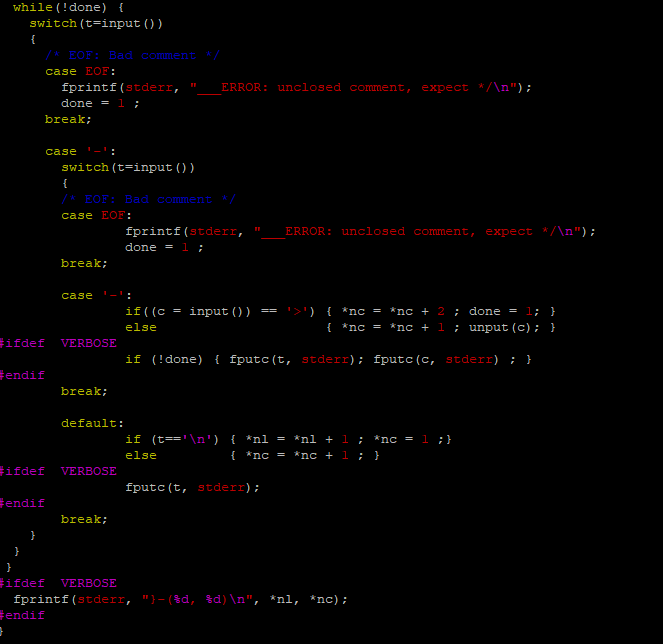
\includegraphics[width=0.75 \textwidth]{Captura1.PNG}}
  \caption{Código de \textit{IgnoraComentarioMultiLinea(&nlin,&ncol)}.}
\end{figure}
 

\newpage
\noindent \\  Otra especificación es que tenemos que tener en cuenta que las etiquetas pueden estar escritas tanto en mayúsculas como en minúsculas como mezcladas (se ve cómo conseguir esto a continuación). Además, para abarcar este amplio campo de posibilidades en casos concretos como "Title"  he usado la opción (\textit{?i:}) gracias a la cual la regla que definas es insensible a mayúsculas y minúsculas (el resto de definiciones se pueden ver en el script). A continuación podemos ver varios ejemplos:

\begin{lstlisting}
    
    SPACE           [ \t]+
    IDENT           [a-zA-Z]+
    ETIQUETA        \<{IDENT}
    TITLE           \<(?i:title)\>
    CIERRETITLE     <\/(?i:title)\>

    
\end{lstlisting}

 \noindent \\ Para obtener el nombre del fichero HTML sobre el que se está aplicando el analizador léxico basta con que en el main se imprima los argumentos correspondientes que se pasan al procedimiento. Para la obtención del título del documento ya se ha dado parte de la solución en párrafos anteriores, solo falta construir una expresión regular como la siguiente:
 
 \begin{lstlisting}
 
 {SPACE}*{IDENT}({SPACE}{IDENT})*/{CIERRETITLE} printf("TITLE:%s\n",yytext);

\end{lstlisting}

\noindent \\ en donde se hace uso del contexto por la derecha para que solo  imprima lo que precede a un cierre de título (\textit{</title>}). La expresión regular representa cero o más espacios seguido de una palabra en mayúsculas, minúsculas o mezcladas y por último seguido de cero o más espacios y palabras (en caso de ser un título que consta de varias palabras). \\

\noindent A continuación se va a mostrar cómo se ha conseguido obtener un resumen estadístico sobre la frecuencia de las distintas etiquetas en el documento estudiado. La expresión regular que he usado es \{ETIQUETA\}[\^{} $>$] y cada vez que se satisfaga dicho patrón se ejecuta el procedimiento \textit{procesamientoEtiquetas()}:

\begin{figure}[H]
  \centering
    \fbox{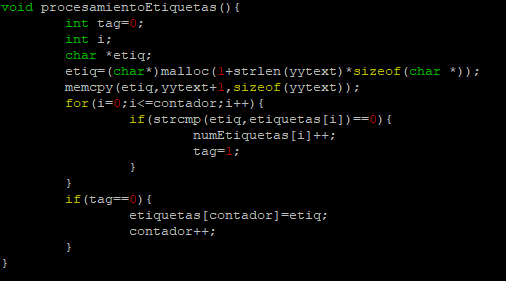
\includegraphics[width=0.75 \textwidth]{Captura2.PNG}}
  \caption{Código de \textit{procesamientoEtiquetas()}.}
\end{figure}

\noindent En el código de la Figura 3 lo único que se hace es almacenar las etiquetas en el array global \textit{etiquetas} en caso de que dichos tags no se hayan almacenado aun, en caso contrario se incrementará en una unidad el número de veces que se ha observado. Además también se nos pide que las ordenemos alfabéticamente y cambiemos a letras minúsculas (función \textit{tolower()}), todo esto se ha conseguido con el siguiente código en C:

\begin{figure}[H]
  \centering
    \fbox{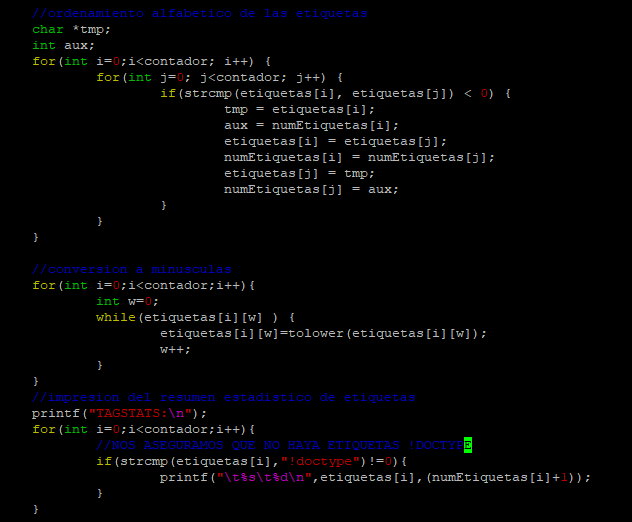
\includegraphics[width=0.75 \textwidth]{Captura3.PNG}}
  \caption{Normalización e impresión del resumen estadístico de etiquetas.}
\end{figure}

\noindent En la figura 4 podemos ver además la consecución de la siguiente especificación de no incluir la etiqueta <!doctype...> en el resumen. Una vez depuradas todas las etiquetas conseguir esto es muy sencillo pues basta con imprimir las etiquetas que cumplan la condición de ser distintas a $"$!doctype$"$. Cierto es que podría haberse usado \textit{Lex} y expresiones regulares para conseguir esto. \\

\noindent A continuación se pide obtener las distintas \textit{URLs} que aparezcan en las etiquetas \textit{<a>, <script> y <link>}. A la hora de resolver esta especificación hay que tener en cuenta que cada etiqueta puede tener uno o más atributos distintos en los que puede haber una \textit{URL}:
\begin{itemize}
    \item \textit{<a>:href}
    \item \textit{<link>:href}
    \item \textit{<script>:src}
\end{itemize}

\noindent Este apartado está claramente pensado para solucionarlo usando condiciones \textit{Start} y usar el contexto izquierdo, pero en mi caso he decidido extraer por completo las etiquetas con sus atributos y procesar posteriormente la cadena para obtener solo el link deseado. Bien es cierto que desde una perspectiva crítica el haber hecho el procesado en C, en vez de haber usado condiciones iniciales, me ha dado una solución más farragosa y menos eficiente. Mediante el uso del contexto izquierdo se podría haber implementado lo siguiente:

\newpage
 \begin{lstlisting}
 
% Start A

%%

{LINKS}.*{HREF}.+   {BEGIN A;}

<A>                 {procesamientoLINKS();
                    BEGIN 0;}

\end{lstlisting}

\noindent \\ Cabe destacar que mi implementación no es del todo correcta porque como en el enunciado dice que se debe mostrar la \textit{URL} sin comillas, había dado por hecho (craso error) que todas las \textit{URLs} se encuentran entre comillas en un fichero HTML. Debido a que me he dado cuenta el mismo día de la entrega que esto no es así siempre, no tengo tiempo suficiente como para cambiar tanto la documentación como la implementación porque, como se va a mostrar a continuación, para la obtención de las \textit{URLs} "limpias" me he basado en encontrar la posición en la que se encuentran las comillas tanto de inicio como de fin para extraer la cadena del medio. A continuación muestro cómo he desarrollado mi solución: 

 \begin{lstlisting}


LINKS   \<((?i:a)|(?i:link))
HREF    (?i:href)

LINKS2 \<(?i:script)
SRC     (?i:src)

%%

{LINKS}.*{HREF}.+/>     {procesamientoLINKS();
                                REJECT;}

{LINKS2}.*{SRC}.+/>     {procesamientoLINKS();
                                REJECT;}

%%

/*
* Almacenamiento de las urls de a, script y link (sin depurar) en arrayEnlaces
*/

void procesamientoLINKS(){
        char *links;
        int indice;
        int tag=1;
        links=(char*)malloc(1+strlen(yytext));
        strcpy(links,yytext);
        arrayEnlaces[contadorEnlaces]=links;
        contadorEnlaces++;
}

\end{lstlisting}

\noindent \\ He vuelto a usar el contexto derecho para eliminar "$>$" (aunque realmente no sería necesario). En las espresiones regulares he tenido en cuenta que las etiquetas tienen atributos con nombres distintos (href, src). La orden \textit{REJECT} sirve para volver y ejecutar distintas alternativas de expresiones regulares que también hayan sido definidas y coincidan con estas (es para que las estadísticas de los tags se obtuviesen de forma correcta). \\
Voy a explicar una de las definiciones de las expresiones regulares (LINKS) que se traduce como <A|<a|<Link|<link|<lInk|...siendo las opciones restantes las combinaciones posibles de mayúsculas y minúsculas sobre la palabra "link". El resto de definiciones son análogas a esta.\\  
Una vez que he obtenido todos los enlaces (sin depurar) he implementado unas líneas de código en C para obtener la \textit{URL} deseada (Figura 5 y 6). 
\bigskip
\begin{figure}[H]
  \centering
    \fbox{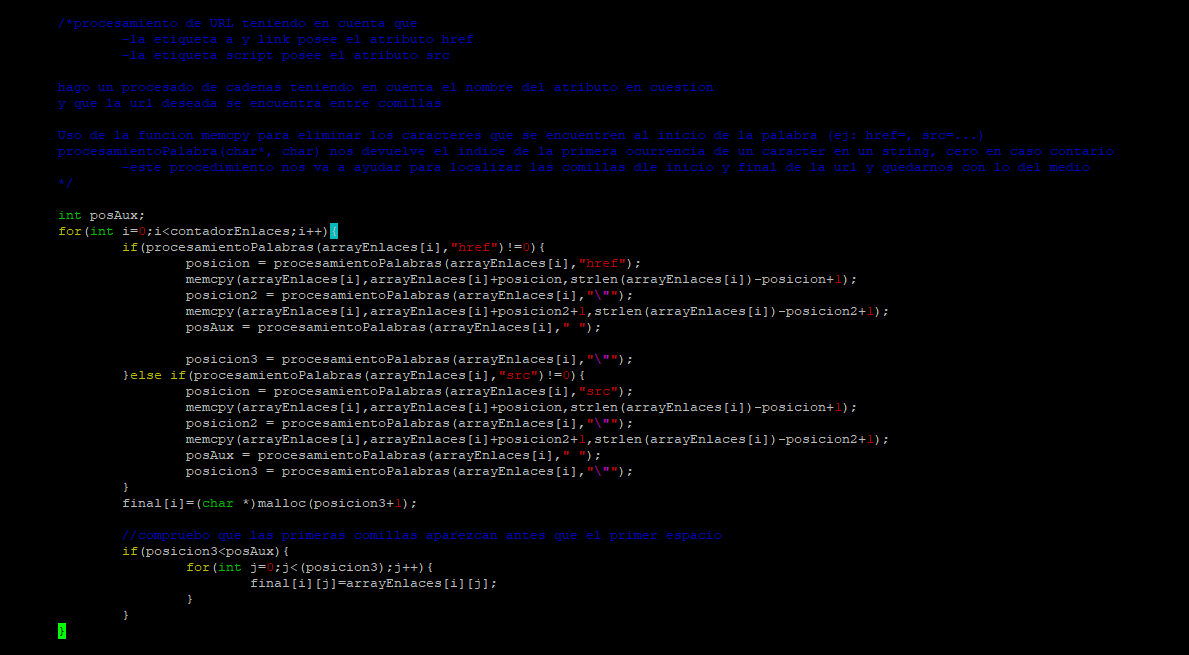
\includegraphics[width=0.85 \textwidth]{url1.PNG}}
  \caption{Procesamiento enlaces(1).}
\end{figure}
\bigskip
\noindent En la Figura 5, para todas las cadenas sin depurar, obtengo la posición donde se encuentra $"$href$"$ o $"$src$"$ y borro todos los caracteres anteriores (para esto uso la función \textit{memcpy}). Posteriormente obtengo el índice donde se encuentran las primeras comillas de la cadena formada en la orden anterior (estas comillas corresponden con comienzo del enlace) y otra vez mediante \textit{memcpy} borro los cararteres anteriores. Por último, de la misma forma, obtengo la posición de las primeras comillas de la cadena creada en el paso previo (corresponden con el final del enlace) y mediante un bucle leo todos los caracteres hasta dicha posición y los almaceno en un array de Strings.\\ Al almacenar los Strings (final del código de la Figura 5) se puede ver que hago una comprobación de si las últimas comillas se encuentran antes que el primer espacio, esto tiene una explicación. Esto es debido a que hay enlaces que no se encuentran entre comillas (cosa que no había previsto) por lo que al ejecutar este código puedo obtener cadenas indeseadas. De esta forma, solo obtengo los links que aparecen entre comillas en el documento HTML pero no obtengo fragmentos indebidos.  
\\ 
\newpage
\noindent Cabe destacar que para estudiar la contención de un substring en un String y obtener la posición se usa la función \textit{procesamientoPalabras(char*,char)}:

\begin{lstlisting}

/*
* Funcion que devuelve la posicion donde se encuentra una subcadena dentro 
* de una cadena
*/
int procesamientoPalabras(char palabra[], char subcadena[]){

        int posicion;
        if(strstr(palabra,subcadena)!=NULL){
                posicion = strstr(palabra,subcadena)-palabra;
                return posicion;
        }else{
                return 0;
        }
}


\end{lstlisting}

\noindent \\ En la Figura 6 lo único que hago es eliminar las \textit{URLs} repetidas:

\begin{figure}[H]
  \centering
    \fbox{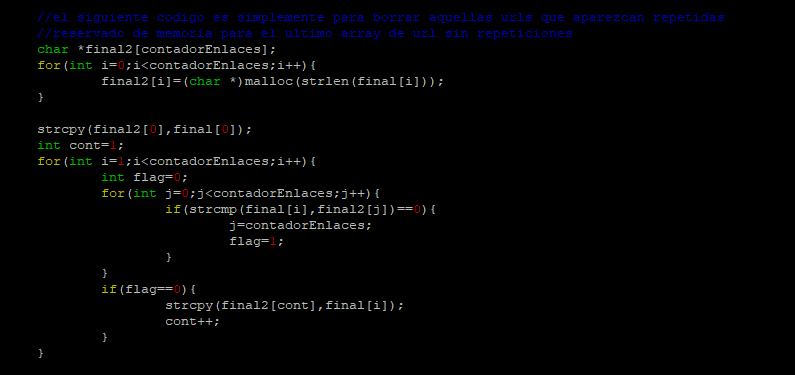
\includegraphics[width=0.85 \textwidth]{url11.PNG}}
  \caption{Procesamiento enlaces(2).}
\end{figure}

\noindent \minibox[frame]{\textbf{NOTA:} En el resultado no se encuentran aquellas \textit{URLs} que no se encuentran entre comillas,\\ debida a la falta de tiempo y todos los cambios que implicaría en mi diseño no he podido cambiarlo.}
\bigskip
\noindent \\ La siguiente especificación consiste también en obtener enlaces pero esta vez de la etiqueta \textit{img}. En esta ocasión me ocurre lo mismo que lo comentado anteriormente en la \textbf{NOTA}. Pese a eso, el funcionamiento es muy similar al caso previo pero esta vez posee más atributos que puedan contener links:

\begin{itemize}
    \item \textit{<img> : src}
    \item \textit{<img> : usemap}
    \item \textit{<img> : longdesc}
\end{itemize}
\newpage
\noindent Es por esto que se han declarado las siguientes expresiones regulares predefinidas, las órdenes correspondientes y el procedimiento que se ejecuta:

\begin{lstlisting}

IMG     \<(?i:img)
LONGDESC (?i:longdesc)
USEMAP   (?i:usemap)

%%

{IMG}.*{SRC}.+/>        {procesamientoIMAGES();
                                REJECT;}

{IMG}.*{LONGDESC}.+/>   {procesamientoIMAGES();
                                REJECT;}

{IMG}.*{USEMAP}.+/>     {procesamientoIMAGES();
                                REJECT;}
                                
%%

/*
* Almacenamiento de las url de imagenes entera(sin depurar) en arrayImagenes
*
*/
void procesamientoIMAGES(){
        char *img;
        img=(char*)malloc(1+strlen(yytext));
        strcpy(img,yytext);
        arrayImagenes[contadorImagenes]=img;
        contadorImagenes++;
}


\end{lstlisting}

\noindent  \\ No voy a detenerme a explicar el código anterior porque es totalmente análogo a la especificación de LINKS. Tanto en la Figura 7 como en la Figura 8 se puede ver la depuración de la cadena hasta la obtención del enlace $"$limpio$"$ y eliminación de duplicados, el procedimiento es exactamente el mismo que el explicado anteriormente, salvando pequeñas diferencias como que el nombre de los atributos es distinto. \\
\bigskip
\begin{figure}[H]
  \centering
    \fbox{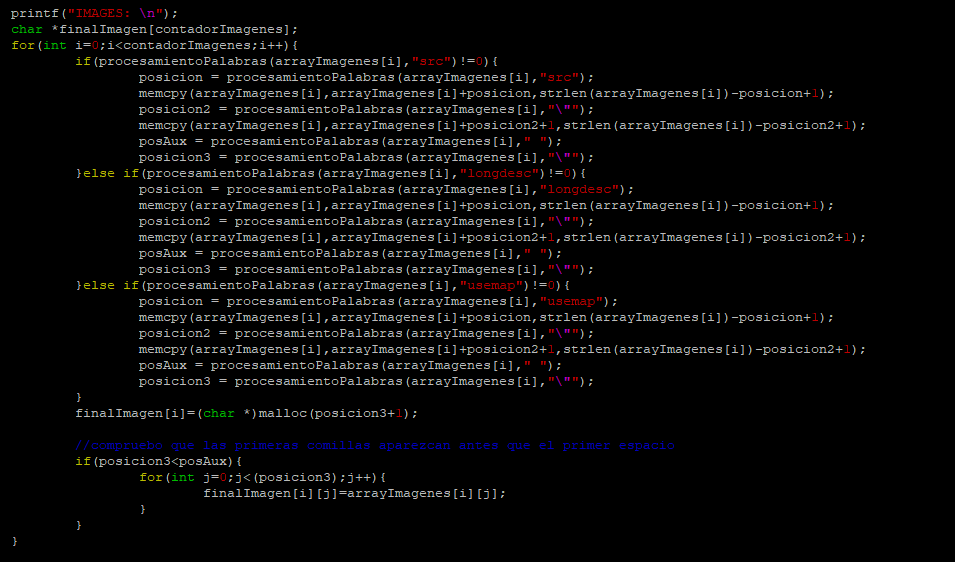
\includegraphics[width=0.95 \textwidth]{url2.PNG}}
  \caption{Procesamiento enlaces de IMG(1).}
\end{figure}

\begin{figure}[H]
  \centering
    \fbox{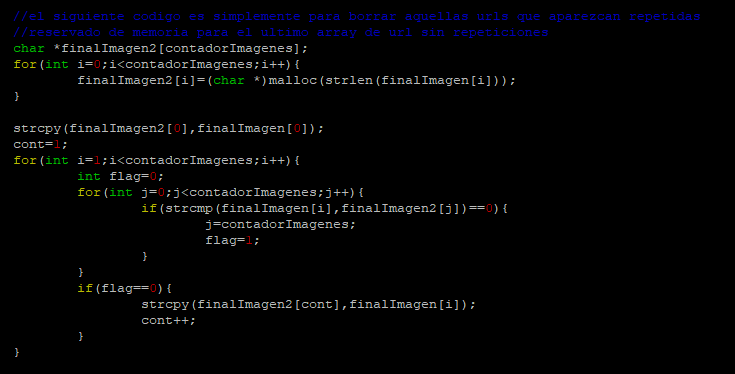
\includegraphics[width=0.85 \textwidth]{Captura7.PNG}}
  \caption{Procesamiento enlaces de IMG(2).}
\end{figure}


\noindent \\ Para completar el analizador léxico se requiere que si existiese, se procesara la información de la etiqueta \textit{<base>} para obtener la \textit{URL} que debería
añadirse a cualquier dirección de enlace (tanto de las imágenes como de enlaces normales). De esta especificación he supuesto entonces que en cada fichero HTML como mucho va a haber un único enlace en \textit{<base>} que será la dirección absoluta. Por esto, cuando encuentre una etiqueta \textit{base} y obtenga dicha dirección de enlace absoluta actualizaré un flag global llamado \textit{Absoluto} y se imprimirá todos los enlaces (igual que en las especificaciones anteriores) pero precedidos de dicho enlace absoluto. Para lograr esto he añadido lo siguiente en las secciones de definiciones,órdenes y rutinas:
\newpage
\begin{lstlisting}

BASE    \<(?i:base)

%%

{BASE}.*{HREF}.+/>      {procesamientoBASE();
                                REJECT;}

%%

/*
* Procedimiento que obtiene la url(sin depurar) del atributo BASE y actualiza la variable global Absoluto
*/
void procesamientoBASE(){

        char *base;
        Absoluto=1;
        base=(char*)malloc(1+strlen(yytext));
        strcpy(base,yytext);
        urlBase[0]=base;
}

\end{lstlisting}

\noindent \\ La explicación del código anterior es análoga a las dadas en apartados anteriores. Aquí cabe resaltar que solo se espera encontrar un enlace en todo el documento HTML y que la variable global \textit{Absoluto} se pone a 1 para que a la hora de imprimir todos los enlaces obtenidos previamente se concatenen a dicha dirección de enlace absoluta. Para lograr esto basta con depurar el enlace igual que en los casos previos e incluir un \textit{if} en función de \textit{Absoluto} (Figura 9 y Figura 10). Finalmente solo hay que imprimir los resultados obtenidos (Figura 11).

\begin{figure}[H]
  \centering
    \fbox{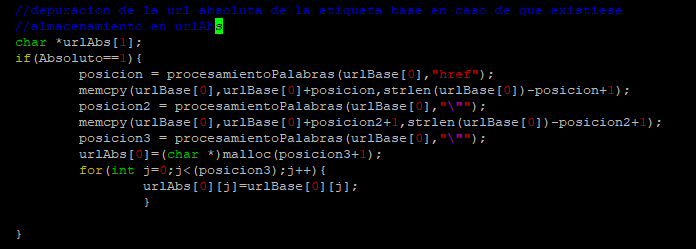
\includegraphics[width=0.85 \textwidth]{Captura8.PNG}}
  \caption{Procesamiento enlace de BASE.}
\end{figure}

\begin{figure}[H]
  \centering
    \fbox{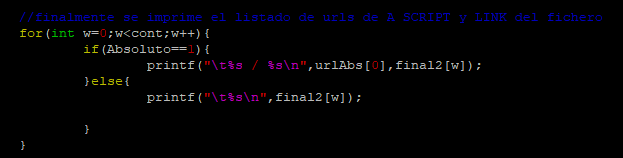
\includegraphics[width=0.85 \textwidth]{Captura9.PNG}}
  \caption{Impresión de los enlaces de A, SCRIPT y LINK.}
\end{figure}

\begin{figure}[H]
  \centering
    \fbox{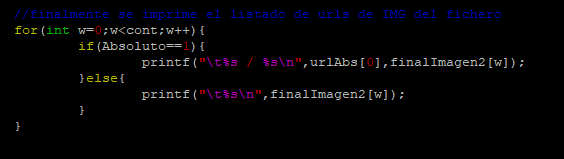
\includegraphics[width=0.85 \textwidth]{Captura10.PNG}}
  \caption{Impresión de los enlaces de IMG.}
\end{figure}

\end{document}
